\documentclass[11pt]{article}
\usepackage[margin=0.9in]{geometry}
\usepackage{amsmath,amssymb,mathtools,bm,booktabs,graphicx,xcolor,microtype}
\usepackage[colorlinks=true,linkcolor=blue,urlcolor=blue,citecolor=blue]{hyperref}
\usepackage{fancyhdr}
\pagestyle{fancy}\fancyhf{}\lhead{Computational Cardiology}\rhead{Planar curve laboratory}\cfoot{\thepage}
\setlength{\headheight}{14pt}\setlength{\parskip}{6pt}\setlength{\parindent}{0pt}
\newcommand{\R}{\mathbb R}\newcommand{\dd}{\,\mathrm d}\newcommand{\rms}{d_{\mathrm{RMS}}}
\hypersetup{pdftitle={Landmarks, correspondence, and ambient flow},pdfauthor={Zan Ahmad},pdfsubject={Planar curve comparison and numerical flow diagnostics}}
\title{Landmarks, correspondence,\protect\\ and ambient flow}\author{Zan Ahmad}\date{Computational Cardiology}
\begin{document}\maketitle
\noindent\href{index.html}{Open the interactive curve laboratory}\quad\href{../../m13/slides.html}{Lecture 13 slides}\quad\href{../../m14/slides.html}{Lecture 14 slides}

The curve laboratory makes three operations distinct: selecting a representation, removing chosen coordinate differences, and deforming the ambient plane. A paired landmark discrepancy gives a finite-dimensional comparison. A velocity field gives a path of ambient transformations. Neither operation by itself computes a geodesic or an elastic distance.

Sections~\ref{sec:arrays}--\ref{sec:diagnostics}, the half-turn calculation, and one experiment form the lecture core. The continuous shape-space discussion in Section~\ref{sec:spaces} and the research comparison in Section~\ref{sec:research} are optional extensions. The six input curves are original analytic examples, not patient outlines. Their coordinates are in millimetres; deformation time is dimensionless.

\section{Ordered landmarks and correspondence}\label{sec:arrays}
A closed polygon is an ordered array
\[
 X=(x_0,\ldots,x_{N-1}),\qquad x_j\in\R^2,
\]
with the closing edge from $x_{N-1}$ to $x_0$. The first point is not duplicated. A point cloud without ordering loses the adjacency needed to form this polygon. A finite polygon also differs from the smooth curve that generated its samples.

The dataset contains a circle, an ellipse, an asymmetric lobed curve, a bean-shaped curve, and posed and scaled copies. For example, the lobed curve is
\[
 r(\theta)=12[1+0.16\cos(3\theta)+0.07\sin(2\theta)],\quad
 c(\theta)=(r(\theta)\cos\theta,0.7r(\theta)\sin\theta).
\]
There are 512 stored angular samples. The laboratory places $N$ landmarks at equal fractions of the stored polygon's perimeter. If $s_k$ is cumulative edge length, $L$ is total length, and $s_k\le jL/N<s_{k+1}$, the new landmark is
\[
 x_j=(1-\alpha)p_k+\alpha p_{k+1},\qquad
 \alpha=\frac{jL/N-s_k}{s_{k+1}-s_k}.
\]
This interpolates the polygon, not an unknown anatomical boundary. An edge of zero length is rejected. Changing $N$ after editing resamples the current polygon; reset returns to the analytic dataset.

For two equally sized arrays, define
\begin{equation}\label{eq:rms}
 \boxed{\rms(X,Y)=\left(\frac1N\sum_{j=0}^{N-1}\|x_j-y_j\|^2\right)^{1/2}.}
\end{equation}
This is the Euclidean norm on $\R^{2N}$ scaled by $N^{-1/2}$, hence a metric on paired arrays. It has length units when the coordinates do. The pairing is part of its definition. Equal arclength fractions do not identify anatomical landmarks.

A cyclic shift uses $y_{(j+k)\bmod N}$; reversing order uses $y_{(k-j)\bmod N}$. These operations change correspondence while leaving the drawn target polygon unchanged. A manually selected shift is not an optimized quotient distance. The laboratory displays the exact chosen pairing and fits no reflection.

\begin{figure}[htbp]\centering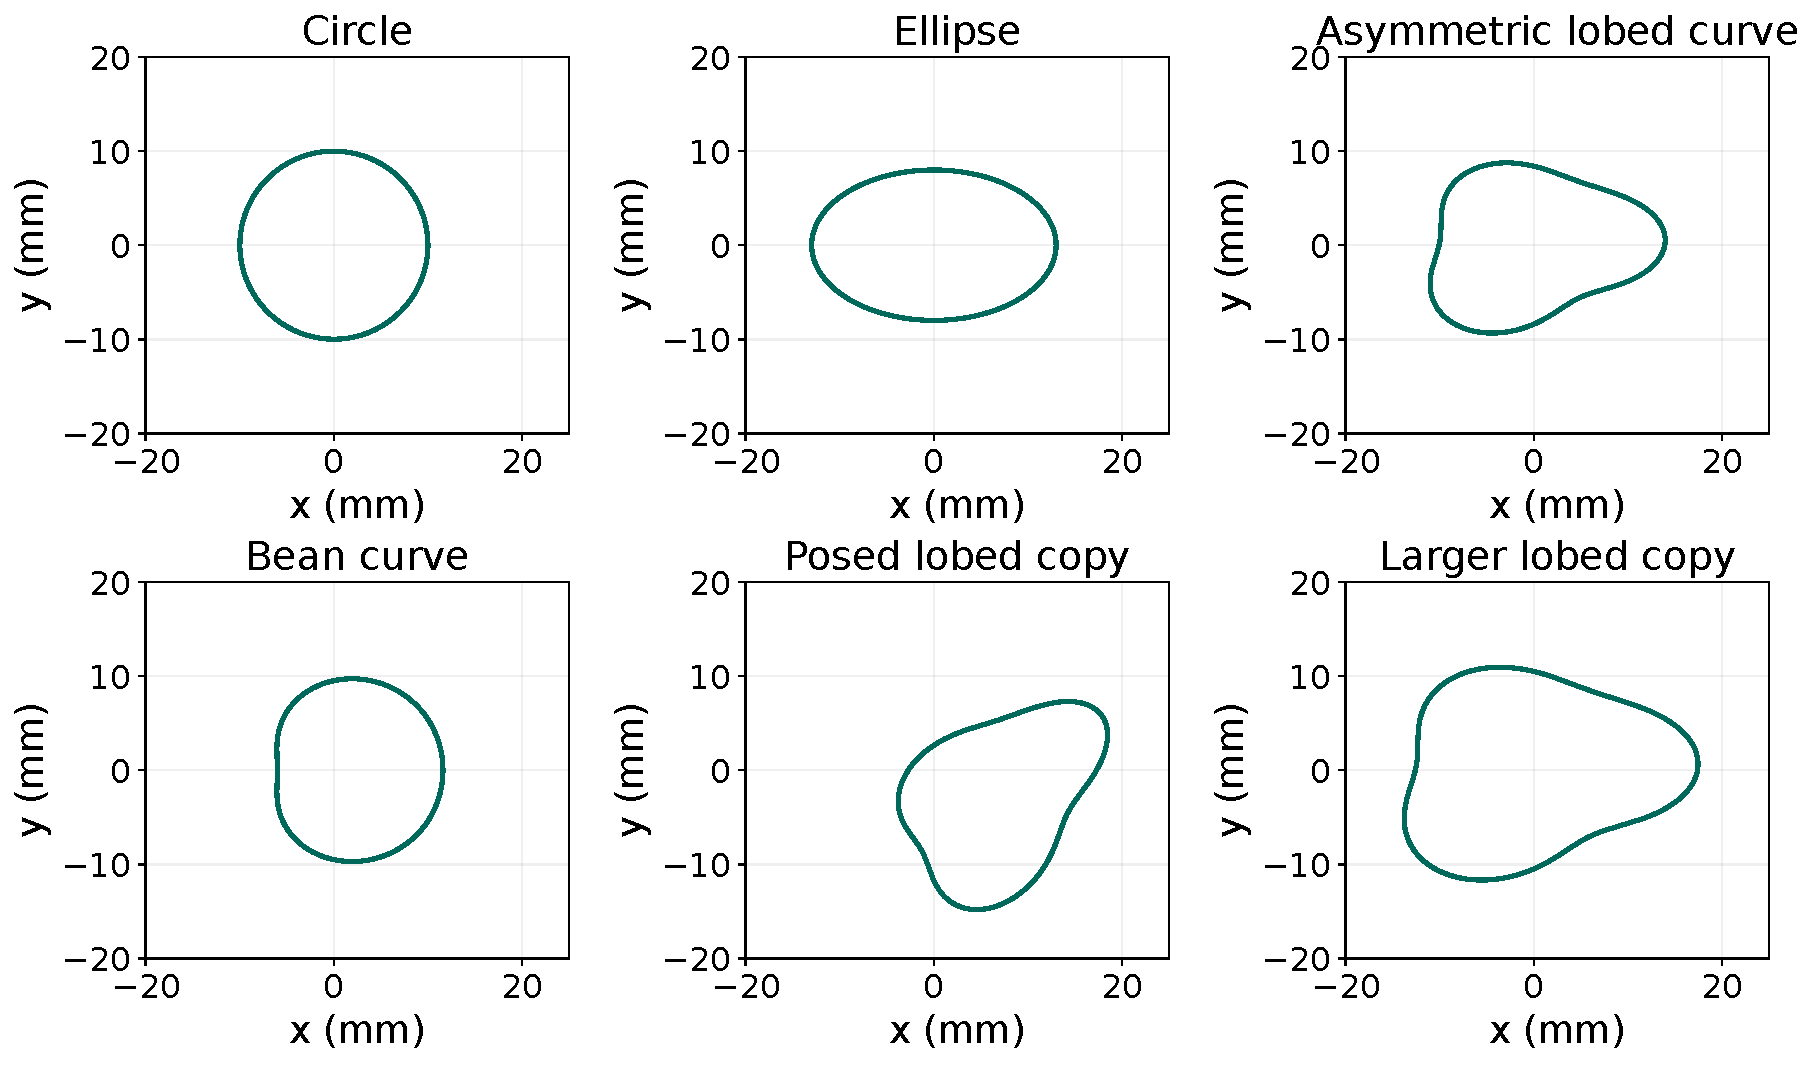
\includegraphics[width=\linewidth]{curated-curves.pdf}\caption{The curated analytic dataset. The posed and larger copies make known limiting cases available. Common axis units retain physical size.}\end{figure}

\section{Centering, proper rotation, and scale}\label{sec:alignment}
The vertex mean is $\bar x=N^{-1}\sum_jx_j$. Subtracting it removes translation. It is not the centroid of the polygon's interior. For a translated copy $Y=X+b$, raw RMS is $\|b\|$ and centered RMS is zero.

Use column-vector rotation
\[
 R(\theta)=\begin{pmatrix}\cos\theta&-\sin\theta\\\sin\theta&\cos\theta\end{pmatrix},\quad \det R=1.
\]
After the chosen centering and normalization operations, the rotation minimizes $\sum_j\|x_j-R(\theta)y_j\|^2$. Let
\[
 a=\sum_j(y_{jx}x_{jx}+y_{jy}x_{jy}),\qquad
 b=\sum_j(y_{jx}x_{jy}-y_{jy}x_{jx}).
\]
Expanding the square shows that minimization is equivalent to maximizing $a\cos\theta+b\sin\theta$. Thus $\theta=\operatorname{atan2}(b,a)$ is a minimizer if $(a,b)\ne(0,0)$. If both vanish, the objective is independent of angle; the code reports nonuniqueness and selects zero. This does not establish anatomical correspondence.

Define the RMS radius about the current origin by
\[
 s_X=\left(\frac1N\sum_j\|x_j\|^2\right)^{1/2}.
\]
Normalization replaces each array by $X/s_X$ and $Y/s_Y$. It removes size and makes the coordinates and RMS dimensionless. With centering enabled, the radius is measured about the vertex mean. With centering disabled, both scale and rotation depend on the chosen coordinate origin. The controls are independent so that this distinction can be tested.

\paragraph{Worked size calculation.}
For centered $Y=1.25X$ with the same correspondence and orientation,
\[
 \rms(X,Y)=0.25s_X.
\]
If $s_X=10\ \mathrm{mm}$, the discrepancy is $2.5\ \mathrm{mm}$. After separate radius normalization, the two arrays agree. The disappearance is a consequence of the declared invariance, not evidence that physical size was irrelevant.

\section{A field fitted to landmark displacements}\label{sec:field}
Write $d_j=y_j-x_j$. A list of displacements says nothing yet about points between or outside the landmarks. We choose a compactly supported radial extension,
\begin{align}
 u(z)&=\sum_{j=0}^{N-1}w_j\,\phi\!\left(\frac{\|z-x_j\|}{\ell}\right),\label{eq:field}\\
 \phi(r)&=(1-r)_+^4(4r+1),\qquad (q)_+=\max(q,0),\quad \ell>0.
\end{align}
This is the $C^2$ Wendland kernel \cite{wendland}. The support radius $\ell$ determines how far each coefficient influences the plane; it is not an elastic metric weight. At the source landmarks, impose
\[
 K W=D,\qquad K_{ij}=\phi(\|x_i-x_j\|/\ell).
\]
Each row of $W$ contains the two components of $w_j$. This is interpolation, not endpoint registration. Distinct source points make the exact positive-definite kernel system nonsingular, but nearby points can make its floating-point solution ill-conditioned. The code checks minimum separation, the matrix infinity-norm condition estimate, and the residual. It disables the field when these guards fail. It adds no hidden regularization term.

For $r_j=\|z-x_j\|/\ell<1$,
\[
 \nabla\phi(r_j)=-\frac{20}{\ell^2}(1-r_j)^3(z-x_j),\qquad
 Du(z)=\sum_j w_j\,[\nabla\phi(r_j)]^{\mathsf T}.
\]
The gradient is zero outside support; the formula also has the correct zero limit at a center. The field is $C^2$, bounded, compactly supported, and globally Lipschitz. For example,
\[
 \|u(z)\|\le\sum_j\|w_j\|,\qquad
 \|Du(z)\|\le L:=\frac{135}{64\ell}\sum_j\|w_j\|,
\]
because $\max_{0\le r\le1}20r(1-r)^3=135/64$. The laboratory limits this conservative $L$ to 40 and the support ratio to $0.6\le\ell/s_X\le2$. These are computational safeguards, not biological bounds. Coordinate units carry into $u$ per unit deformation time; $Du$ is per unit deformation time.

\section{Coordinate interpolation and ambient flow}\label{sec:maps}
The coordinate map treats $u$ as a displacement:
\begin{equation}\label{eq:naive}
 F_t(z)=z+t\,u(z),\qquad 0\le t\le1.
\end{equation}
Since $u(x_j)=y_j-x_j$, each landmark follows the straight segment
\[
 F_t(x_j)=(1-t)x_j+ty_j,
\]
and reaches $y_j$ at $t=1$. The same field acts on the ambient grid. Smoothness of $u$ alone does not make $F_t$ injective.

The flow instead treats the same function as a stationary velocity:
\begin{equation}\label{eq:flow}
 \dot\Phi_t(z)=u(\Phi_t(z)),\qquad \Phi_0(z)=z.
\end{equation}
It reevaluates velocity at the moving position. The bounded Lipschitz field has unique trajectories for every finite positive or negative time. Uniqueness prevents trajectories from meeting; the inverse is obtained by integrating backward. Its differentiability gives an ambient diffeomorphism. This applies to the exact flow; a finite numerical approximation requires separate checks.

The two maps initially agree to first order, but not generally later:
\[
 \Phi_t(z)=z+t u(z)+\frac{t^2}{2}Du(z)u(z)+O(t^3).
\]
Consequently, $\Phi_1(x_j)$ need not equal $y_j$. The laboratory reports the flow endpoint RMS separately from the interpolation residual. Minimizing an initial velocity fit is not minimizing endpoint mismatch. There is no endpoint optimizer, path-energy minimizer, or geodesic claim here.

\begin{figure}[htbp]\centering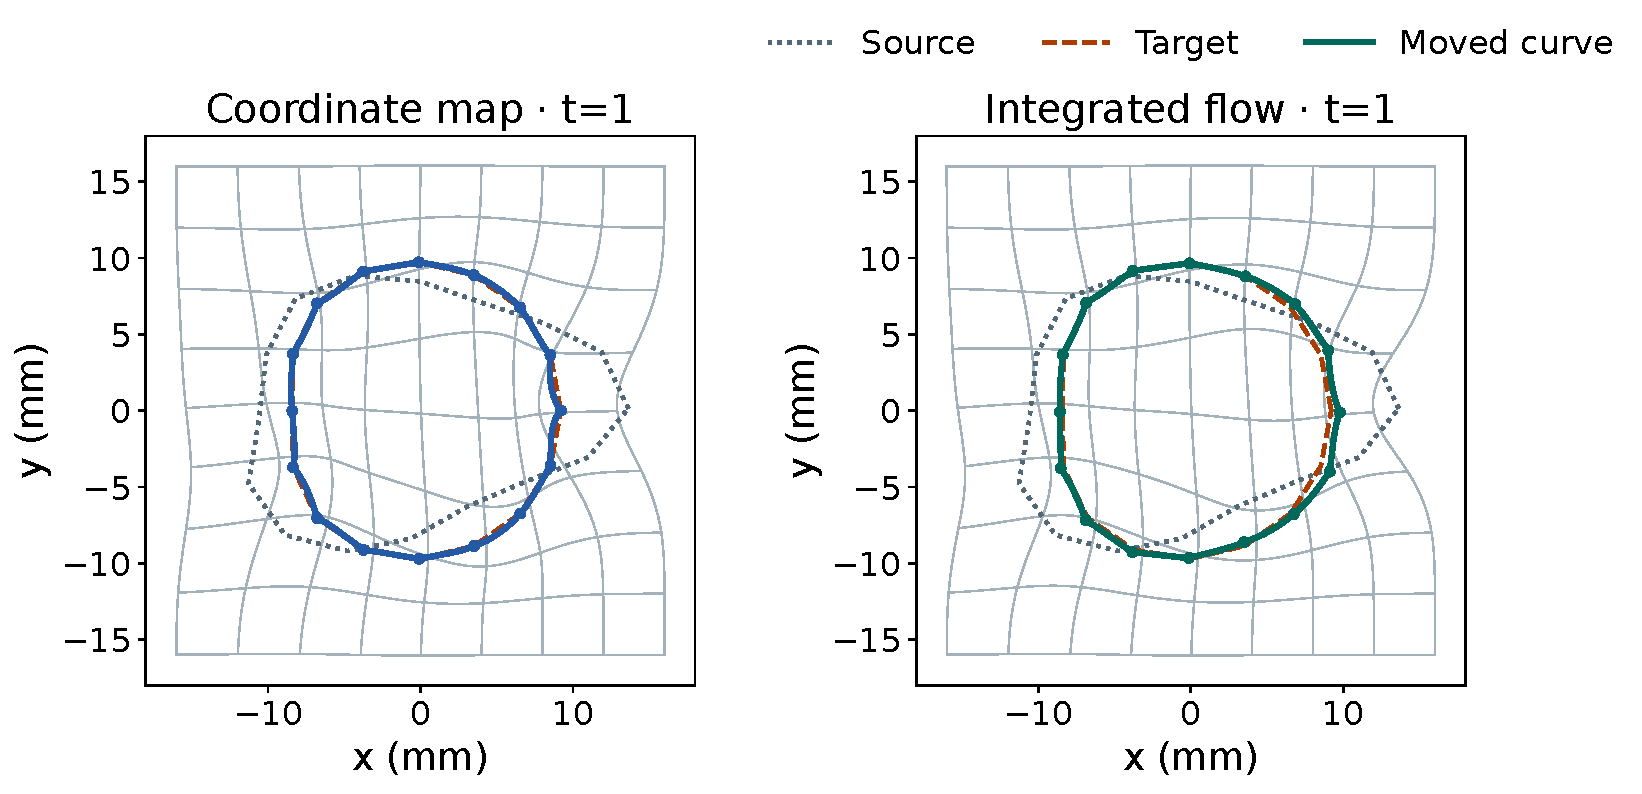
\includegraphics[width=\linewidth]{flow-comparison.pdf}\caption{Default lobed-to-bean comparison at $t=1$. The coordinate map reaches the target landmarks, whereas the integrated stationary flow has a nonzero endpoint mismatch. The grey grid undergoes the same ambient transformation as the sampled source curve.}\end{figure}

\paragraph{Half-turn correspondence.}
For an even number of equally spaced circle landmarks, shift target indexing by $N/2$ and disable rotation fitting. Then $y_j=-x_j$, so
\[
 F_t(x_j)=(1-2t)x_j.
\]
All landmarks coincide at $t=1/2$. For the landmark polygon, signed area is $(1-2t)^2$ times its initial area, so area vanishes at the collapse but is positive again afterward. Positive endpoint area would miss the intermediate singularity. The interpolated ambient field is only constrained at landmarks; its image between those landmarks need not collapse to the same point.

The exact flow cannot reproduce this finite-time collision. A failure to reach the target does not contradict its topology-preserving construction. This example also shows why a bad pairing can be more consequential than a small numerical integration error.

\section{Jacobian evolution and numerical evidence}\label{sec:diagnostics}
For the coordinate map,
\[
 DF_t(z)=I+tDu(z).
\]
The laboratory samples its determinant. A nonpositive value detects a singularity or local orientation reversal at that sample. Positive values at a finite set do not establish global injectivity, nor rule out a fold between samples.

For the exact flow, differentiate Equation~\eqref{eq:flow} with respect to its initial point. With $A(t,z)=D\Phi_t(z)$,
\begin{equation}\label{eq:variation}
 \dot A=Du(\Phi_t(z))A,\qquad A(0,z)=I.
\end{equation}
Jacobi's determinant identity gives
\[
 \frac{\mathrm d}{\mathrm dt}\log\det A=\nabla\cdot u(\Phi_t(z)),\qquad
 \boxed{\det A(t,z)=\exp\!\left(\int_0^t\nabla\cdot u(\Phi_s(z))\dd s\right)>0.}
\]
Orientation preservation does not mean area preservation: the latter would require zero divergence. The implementation integrates position, the four entries of $A$, and a separate scalar $\lambda$ satisfying $\dot\lambda=\nabla\cdot u(\Phi_t)$, $\lambda(0)=0$.

Classical four-stage RK4 advances this augmented system. The finer run stores 65 times. We compare runs at $\Delta t$ and $\Delta t/2$: the finer run uses twice as many steps. The default experiment uses 128 and 256 steps, respectively. The kernel is only finitely smooth across its support boundary, so a nominal method label is not a substitute for measured refinement. The displayed tests are:
\begin{enumerate}
\item the maximum positional difference between the two time steps over the displayed sample locations;
\item forward-then-backward discrepancy at the source landmarks;
\item the discrepancy between $\det A$ and $\exp\lambda$;
\item the smallest computed determinant over all cached sample states.
\end{enumerate}
The first two position tolerances are $2\times10^{-5}s_X$, and the relative determinant-identity tolerance is $10^{-4}$. They are diagnostic tolerances, not an error bound proved for every initial point. Samples include grid nodes, source-edge samples and landmarks. The displayed curve is a sampled image of source edges, whereas the area and strict crossing count use the landmark polygon. Chords can miss curvature, tangencies or degeneracies. Refining spatial samples is a separate experiment from refining the ODE time step.

\begin{figure}[htbp]\centering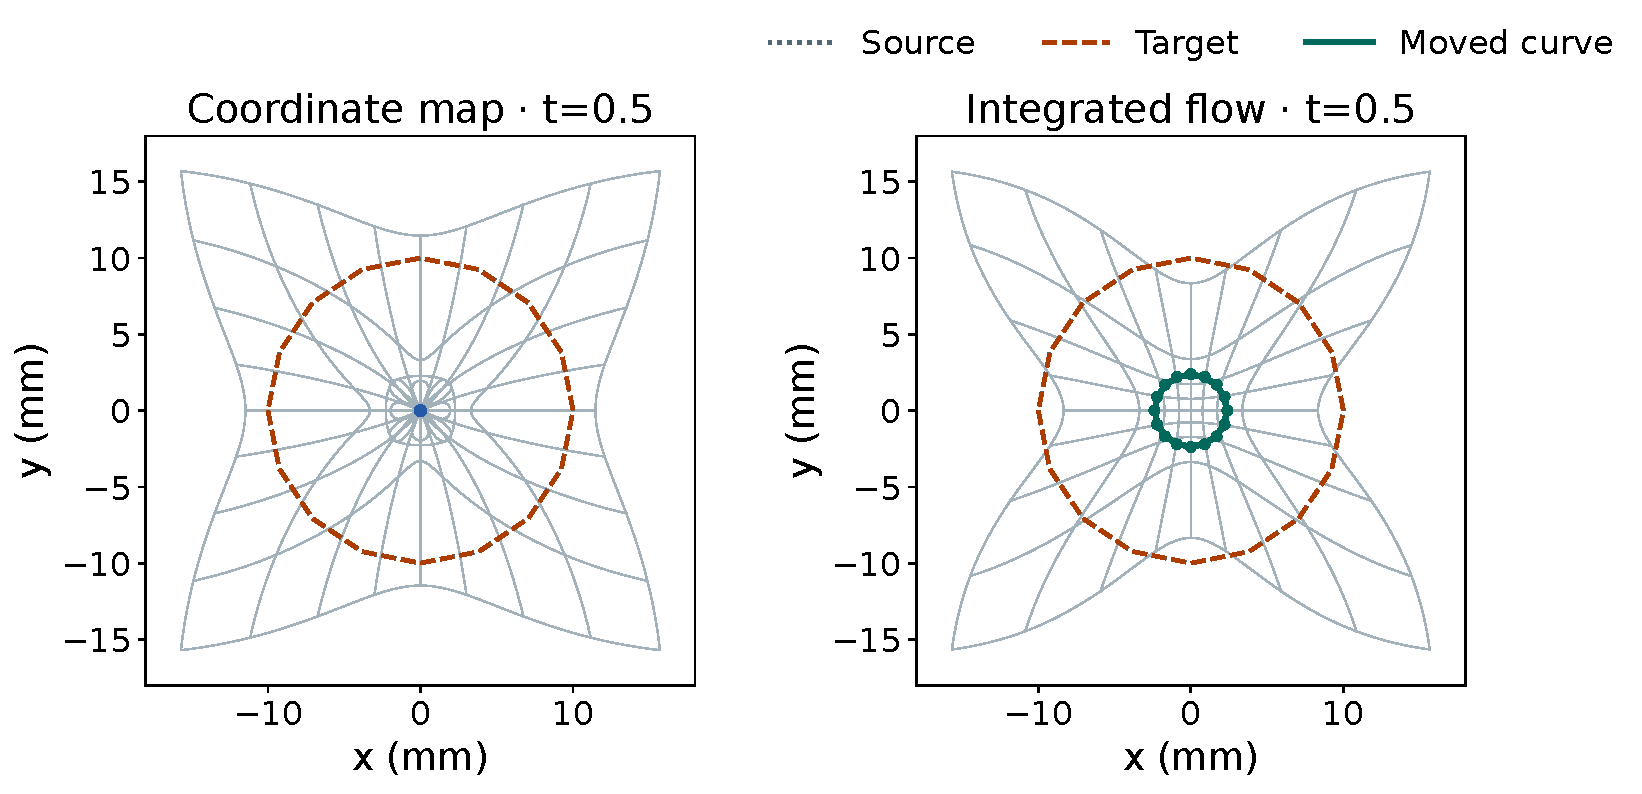
\includegraphics[width=\linewidth]{landmark-collapse.pdf}\caption{Half-turn correspondence at $t=1/2$. The coordinate-map landmarks collapse; the ambient interpolation between them can form small loops. The exact flow keeps trajectories distinct. Its numerical approximation is accompanied by sampled Jacobian and time-refinement diagnostics.}\end{figure}

\section{From configurations to shape spaces (optional)}\label{sec:spaces}
Distinct labelled landmarks form the open configuration space
\[
 \operatorname{Conf}_N(\R^2)=\{X\in(\R^2)^N:x_i\ne x_j\text{ for }i\ne j\},
\]
a smooth manifold of dimension $2N$. Distinct vertices do not guarantee a simple polygon: nonadjacent edges may cross. The laboratory checks strict segment intersections and reports them without treating that test as a complete geometric certificate.

Centering selects a linear subspace with two fewer dimensions. Unit RMS radius selects a sphere within it. Removing proper rotations or cyclic labels forms equivalence classes, rather than merely deleting another array column. Symmetries of an unlabelled curve can produce nonunique representatives and quotient singularities; one should not call every such quotient a single Euclidean manifold.

A continuous closed curve is a map $c:S^1\to\R^2$. An immersion has $\partial_\theta c\ne0$ everywhere, while an embedding is also injective. Its tangent perturbations are vector fields along the curve. Removing parametrization means identifying $c$ with $c\circ\gamma$ for suitable diffeomorphisms $\gamma:S^1\to S^1$. A cyclic shift of $N$ indices is only a finite convention, not optimization over all such reparametrizations.

Two different actions now appear. A reparametrization changes the labels along a fixed geometric image. An ambient diffeomorphism changes the image by $c\mapsto\Phi\circ c$. Confusing these actions confuses correspondence with deformation. The ODE model here supplies the second action after a particular finite pairing has been selected.

\section{Relation to geometric registration (optional)}\label{sec:research}
Beg, Miller, Trouv\'e and Younes \cite{beg} use sufficiently regular velocity fields to generate diffeomorphisms and optimize a variational registration objective. Our prescribed stationary field illustrates the distinction between a displacement map and an integrated flow, without implementing their optimization or inferring a shortest-path metric.

Ahmad and colleagues \cite{ahmad} compare three-dimensional appendage surfaces using a second-order Sobolev metric, relaxed endpoint matching and a varifold discrepancy. Their optimized path energy and endpoint discrepancy have separate roles. A schematic objective is
\[
 \int_0^1G_{c(t)}(\dot c(t),\dot c(t))\dd t
 +\beta\,\Gamma(c(1),c_{\mathrm{target}}).
\]
This laboratory supplies neither that metric $G$, nor the varifold term $\Gamma$, nor an optimization over paths. It uses paired planar RMS, an interpolating kernel field, and a numerical initial-value problem. The research paper provides geometric context, not a validation of the analytic curves or of any clinical conclusion from them.

\section{Exercises and computational record}\label{sec:practice}
\begin{enumerate}
\item Let $X=((0,0),(3,0),(0,3))$ mm and $Y=X+(2,-1)$ mm. Compute both vertex means, raw RMS and centered RMS. For this triangle the vertex mean equals its area centroid. Explain why vertex averaging is not a general definition of a polygon's area centroid. Then derive the residual for a centered scaled copy $Y=aX$, $a>0$.
\item For equally spaced even-$N$ circle landmarks of radius $R$, use the half-turn correspondence. Derive the RMS to the paired target at time $t$, the landmark-polygon area factor, and the collapse time. Explain why a positive final signed area misses this failure. Use uniqueness of the ODE flow to explain why distinct trajectories cannot produce the same finite-time collision.
\item Consider the analytic shear field $u(x,y)=(ay,0)$. Solve its flow and Jacobian exactly. Compare with $F_t$. Then consider $u(x,y)=(-\omega y,\omega x)$. Derive the exact flow and $\det DF_t$. Explain why agreement for a shear does not imply agreement for rotation. These are analytic verification fields, not fitted compact-support fields.
\item Reset the laboratory. Record $N$, correspondence, alignment toggles, support radius, paired RMS, flow endpoint RMS, time-refinement gap and minimum sampled Jacobian. Change just one control and repeat. State which differences are mathematical model choices and which quantities diagnose numerical error. Run and report one limiting test, such as the identity case. Give one claim that positive sampled Jacobians cannot establish.
\end{enumerate}

Download the experiment JSON to retain raw edited coordinates and controls. Save it next to \texttt{companion.py} and \texttt{curves.json}, then run
\begin{verbatim}
python companion.py --experiment shape-experiment.json --out results.json
\end{verbatim}
The default run uses the lobed and bean curves with 16 landmarks. Python and JavaScript implement the same finite model; their comparison is an implementation check. No MATLAB execution or equivalence is claimed.

\noindent\href{index.html}{Return to the laboratory}\quad\href{../../m13/notes.pdf}{Lecture 13 notes}\quad\href{../../m14/notes.pdf}{Lecture 14 notes}
\begin{thebibliography}{9}
\bibitem{wendland} H. Wendland. Piecewise polynomial, positive definite and compactly supported radial functions of minimal degree. \emph{Advances in Computational Mathematics} 4, 389--396 (1995). \href{https://doi.org/10.1007/BF02123482}{doi:10.1007/BF02123482}.
\bibitem{beg} M. F. Beg, M. I. Miller, A. Trouv\'e, L. Younes. Computing large deformation metric mappings via geodesic flows of diffeomorphisms. \emph{International Journal of Computer Vision} 61, 139--157 (2005). \href{https://doi.org/10.1023/B:VISI.0000043755.93987.aa}{doi:10.1023/B:VISI.0000043755.93987.aa}.
\bibitem{ahmad} Z. Ahmad, M. Yin, Y. Sukurdeep, N. Rotenberg, E. Kholmovksi, N. Trayanova. A computational pipeline for clustering left atrial appendage morphology via elastic shape analysis. \emph{Computers in Biology and Medicine} 196, 110905 (2025). \href{https://doi.org/10.1016/j.compbiomed.2025.110905}{doi:10.1016/j.compbiomed.2025.110905}.
\end{thebibliography}
\end{document}
